% Exam Template for UMTYMP and Math Department courses
%
% Using Philip Hirschhorn's exam.cls: http://www-math.mit.edu/~psh/#ExamCls
%
% run pdflatex on a finished exam at least three times to do the grading table on front page.
%
%%%%%%%%%%%%%%%%%%%%%%%%%%%%%%%%%%%%%%%%%%%%%%%%%%%%%%%%%%%%%%%%%%%%%%%%%%%%%%%%%%%%%%%%%%%%%%

% These lines can probably stay unchanged, although you can remove the last
% two packages if you're not making pictures with tikz.
\documentclass[11pt]{exam}
\RequirePackage{amssymb, amsfonts, amsmath, latexsym, verbatim, xspace, setspace}
\RequirePackage{tikz, pgflibraryplotmarks}

% By default LaTeX uses large margins.  This doesn't work well on exams; problems
% end up in the "middle" of the page, reducing the amount of space for students
% to work on them.
\usepackage[margin=1in]{geometry}
\usepackage{afterpage}
\usepackage{changepage}

% Here's where you edit the Class, Exam, Date, etc.
\newcommand{\class}{CS 143A}
\newcommand{\term}{Fall 2019}
\newcommand{\examnum}{Midterm}
\newcommand{\examdate}{11/13/2019}
\newcommand{\timelimit}{11:00pm - 11:50pm}

% For an exam, single spacing is most appropriate
\singlespacing
% \onehalfspacing
% \doublespacing

% For an exam, we generally want to turn off paragraph indentation
\parindent 0ex

\begin{document} 

% These commands set up the running header on the top of the exam pages
\pagestyle{head}
\firstpageheader{}{}{}
\runningheader{\class}{\examnum\ - Page \thepage\ of
\numpages}{\fbox{\rule{2in}{0pt}\rule[-0.5ex]{0pt}{5ex}}}
\runningheadrule

\begin{flushright}
\begin{tabular}{p{2.8in} r l}
%\textbf{\class} & \textbf{Name (Print):} & \makebox[2in]{\hrulefill}\\
  \textbf{\class} & \textbf{Name (Print):} &
  \fbox{\rule{2in}{0pt}\rule[-0.5ex]{0pt}{5ex}}\\
   \textbf{\term} & \textbf{Seat:} &
    \fbox{\parbox{0pt}{SEAT}\rule{2in}{0pt}\rule[-0.5ex]{0pt}{5ex}}\\
\textbf{\examnum} & \textbf{Left person:} &
    \fbox{\rule{2in}{0pt}\rule[-0.5ex]{0pt}{5ex}}\\
\textbf{\examdate} & \textbf{Right person:} &
    \fbox{\rule{2in}{0pt}\rule[-0.5ex]{0pt}{5ex}}\\
\textbf{Time Limit: \timelimit} & & \\
\end{tabular}\\
\end{flushright}
\rule[1ex]{\textwidth}{.1pt}




%\begin{minipage}[t]{3.7in}
%\vspace{0pt}
\begin{itemize}

\item \textbf{Don't forget to write your name on this exam.} 

\item \textbf{This is an open book, open notes exam. But no online or 
    in-class chatting.  } 

    
\item \textbf{Ask us if something is confusing in the questions.}

\item \textbf{Organize your work}, in a reasonably neat and coherent way, in
the space provided. Work scattered all over the page without a clear ordering will 
receive very little credit.  

\item \textbf{Mysterious or unsupported answers will not receive full
credit}.  A correct answer, unsupported by explanation will receive no credit; 
an incorrect answer supported by substantially correct explanations might still 
receive partial credit.

\item If you need more space, use the back of the pages; clearly indicate when you have done this.
\end{itemize}

%Do not write in the table to the right.
%\end{minipage}
%\hfill

%\begin{minipage}[t]{2.3in}
%\vspace{0pt}
%\cellwidth{3em}
%\gradetablestretch{2}
\vqword{Problem}
\addpoints % required here by exam.cls, even though questions haven't started yet.	
\gradetable[v]%[pages]  % Use [pages] to have grading table by page instead of question

%\end{minipage}
\newpage % End of cover page

%%%%%%%%%%%%%%%%%%%%%%%%%%%%%%%%%%%%%%%%%%%%%%%%%%%%%%%%%%%%%%%%%%%%%%%%%%%%%%%%%%%%%
%
% See http://www-math.mit.edu/~psh/#ExamCls for full documentation, but the questions
% below give an idea of how to write questions [with parts] and have the points
% tracked automatically on the cover page.
%
%
%%%%%%%%%%%%%%%%%%%%%%%%%%%%%%%%%%%%%%%%%%%%%%%%%%%%%%%%%%%%%%%%%%%%%%%%%%%%%%%%%%%%%

\begin{questions}

% Basic question
\addpoints
\question Calling conventions 

\begin{parts}
 
\part[5] Below is the source code and a disassembly of a simple C pogram:



\begin{verbatim}
 int foo(int a) {                1. 00000000 <foo>:
         a++;                    2.   0:	push   ebp
         return a;               3.   1:	mov    ebp,esp
 }                               4.   3:	add    DWORD PTR [ebp+0x8],0x1
                                 5.   7:	mov    eax,DWORD PTR [ebp+0x8]
 int main(int ac, char **av)     7.   a:	pop    ebp
 {                               8.   b:	ret    
     return foo(1);              9.
 }                               10. 0000000c <main>:
                                 11.   ...
                                 12.   f:	push   0x1   <---- eip
                                 13.  11:	call   foo
                                 14.  16:        ...

\end{verbatim}

The CPU is about to execute the push instruction at line 12 (address 0xf) of the disassembly. 
Draw the stack and how it changes with every instruction of this program until \texttt{foo()} returns, 
i.e., lines 12, 13, 1-8, and 14 (i.e., figures for the stack in 9 different states). 

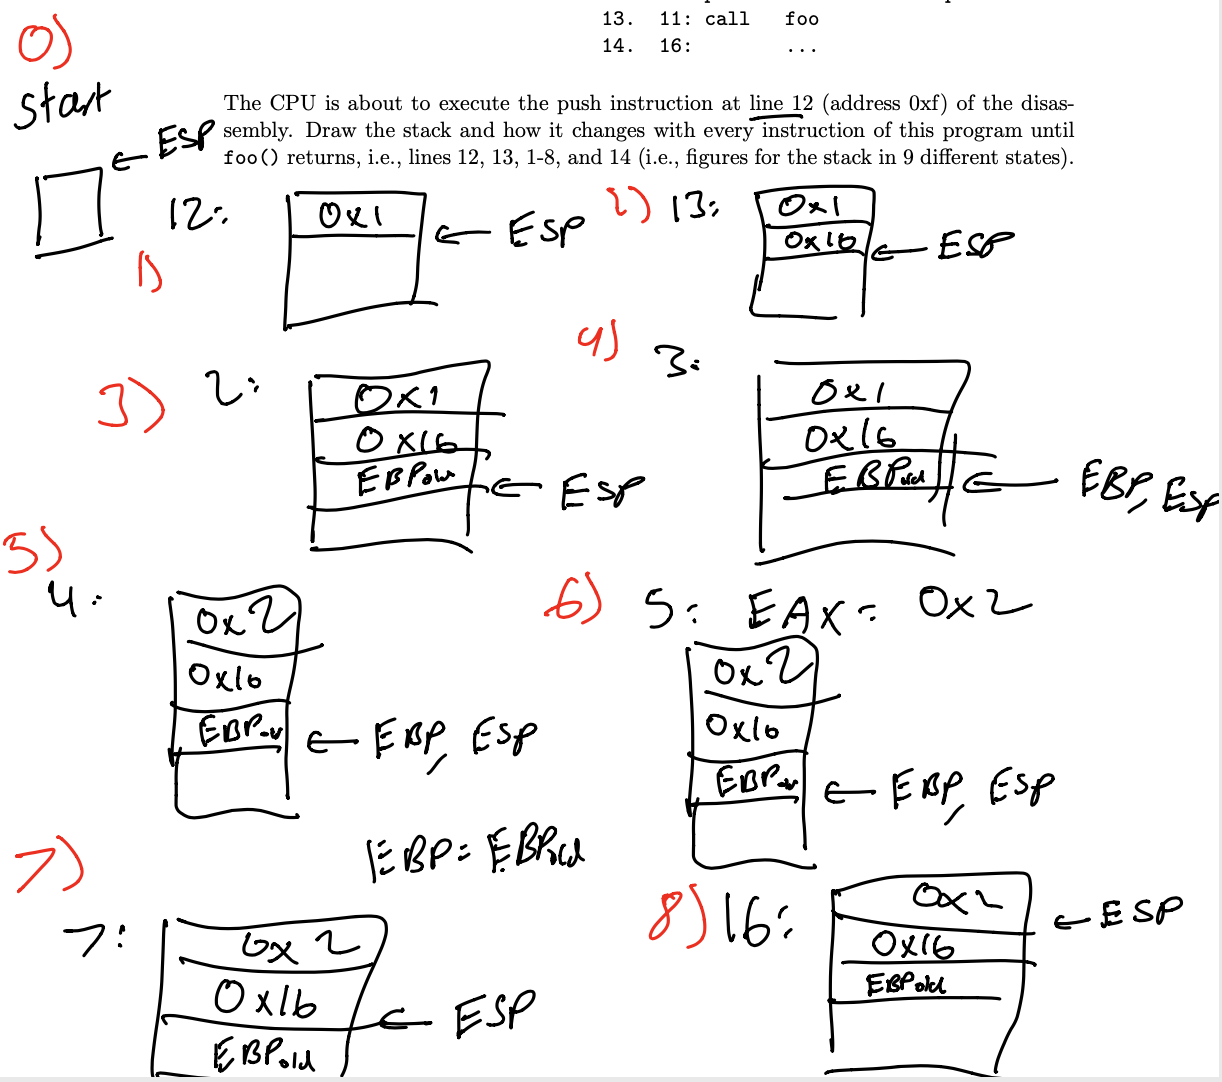
\includegraphics[width=0.5\columnwidth]{figs/point-1a}
\vfill

\part[10] Imagine your CPU is identical to x86 but does not have \texttt{call} and \texttt{ret} instructions. How will you implement 
	the assembly code above (i.e., your code should support recursive invocation of functions)? 

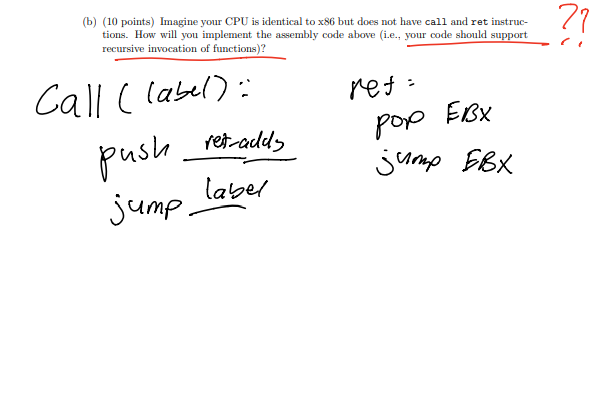
\includegraphics[width=0.5\columnwidth]{figs/point-1b}
\vfill


\end{parts} 

% Basic question
\addpoints

\newpage
\question Basic page tables.

\begin{parts}
\iffalse

\part[5] 

Image you're running the system with the following page table. Now you change the user changes 	
Assume that the

Page Directory Page is at physical address 0x0, and the Page Table Page is at
physical address 0x1000 (which is PPN 0x1). 

Page Directory Page:

\begin{verbatim}
PDE 0: PPN=0x1, PTE_P, PTE_U, PTE_W
PDE 1: PPN=0x2, PTE_P, PTE_U, PTE_W
\end{verbatim}

... all other PDEs are zero

The Page Table Page at the physical address 0x1000:

\begin{verbatim}
PTE 0: PPN=0x1, PTE_P, PTE_U, PTE_W
PTE 1: PPN=0x2, PTE_P, PTE_U, PTE_W
PTE 2: PPN=0x3, PTE_P, PTE_U, PTE_W
\end{verbatim}

... all other PTEs are zero

The Page Table Page at the physical address 0x2000:

\begin{verbatim}
PTE 0: PPN=0x0, PTE_P, PTE_U, PTE_W
PTE 1: PPN=0x4, PTE_P, PTE_U, PTE_W
\end{verbatim}


\fi

\part[5] 

	Which physical address is accessed by the following \texttt{mov} instruction? 
	
\begin{verbatim}
mov    eax, DWORD PTR [ebx+0x8]
\end{verbatim}

Here the \texttt{ebx} register contains 0x1000, and the 
data segment is configured to have the base of 0x1000. 

Page Directory Page:

\begin{verbatim}
PDE 0: PPN=0x1, PTE_P, PTE_U, PTE_W
PDE 1: PPN=0x2, PTE_P, PTE_U, PTE_W
PDE 2: PPN=0x3, PTE_P, PTE_U, PTE_W
\end{verbatim}

... all other PDEs are zero

The Page Table Page at the physical address 0x1000:

\begin{verbatim}
PTE 0: PPN=0x0, PTE_P, PTE_U, PTE_W
PTE 1: PPN=0x1, PTE_P, PTE_U, PTE_W
PTE 2: PPN=0x2, PTE_P, PTE_U, PTE_W
\end{verbatim}

The Page Table Page at the physical address 0x2000:

\begin{verbatim}
PTE 0: PPN=0x4, PTE_P, PTE_U, PTE_W
PTE 1: PPN=0x5, PTE_P, PTE_U, PTE_W
PTE 2: PPN=0x6, PTE_P, PTE_U, PTE_W
\end{verbatim}

The Page Table Page at the physical address 0x3000:

\begin{verbatim}
PTE 0: PPN=0x7, PTE_P, PTE_U, PTE_W
PTE 1: PPN=0x8, PTE_P, PTE_U, PTE_W
PTE 2: PPN=0x9, PTE_P, PTE_U, PTE_W
\end{verbatim}
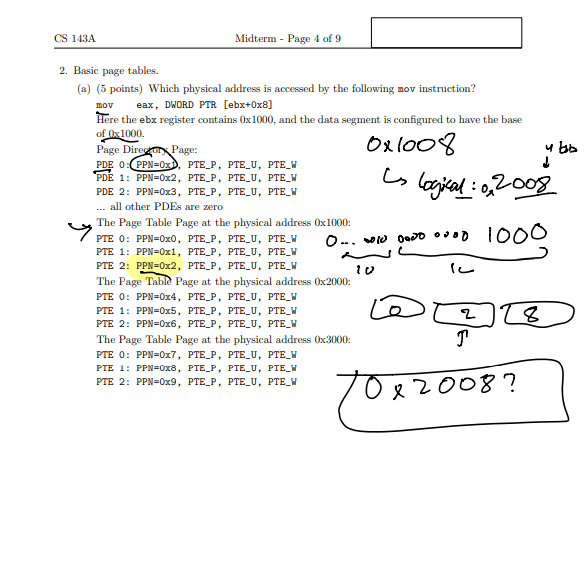
\includegraphics[width=0.5\columnwidth]{figs/point-2a}
\newpage

\part[5] Draw a page table (you can use the format similar to the previous
question) that maps virtual (or if you want to be more specific, linear) 
addresses 2GB (0x8000000) to 2GB + 16KB (0x8004000) to physical addresses 
0 to 16KB (0x4000). 

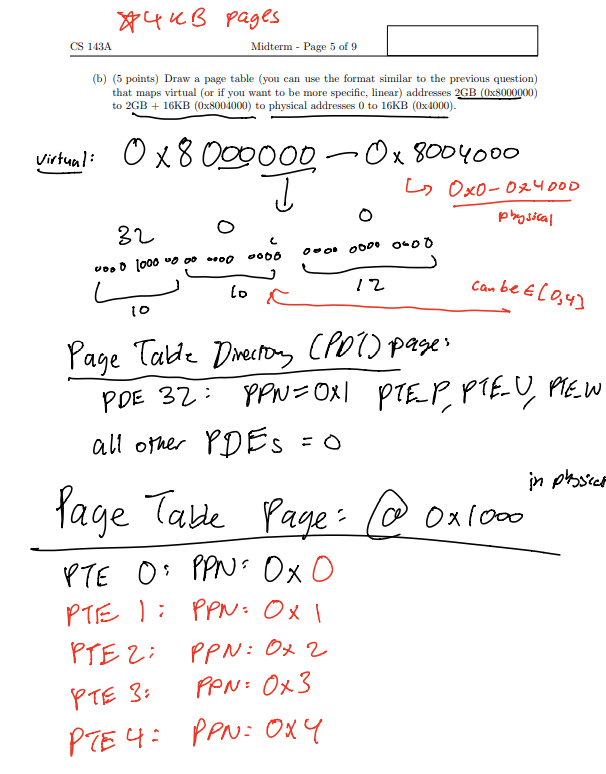
\includegraphics[width=0.5\columnwidth]{figs/point-2b}
\vfill

\end{parts} 


\addpoints

\newpage

\question Xv6 boot

\begin{parts} 

\part[10] When xv6 boots, the boot loader loads the xv6 kernel at the physical
	address 0x10000 (1MB). The boot loader jumps to the entry point of the kernel ELF
	file which is linked to be at 0x10000c. The first thing the xv6 kernel does is it sets up the boot-time
	page table that maps two regions of vistual memory (0-4MB and
	2GB-(2GB+4MB)) to the physical range 0 to 4MB, and then jumps to the C \texttt{main()} function that runs 
	in the 2GB-(2GB+4MB) range. This seems counter-intuitive: the kernel seems to
	be able to run at two virtual address ranges: 0-4MB and 2GB-(2GB+4MB)---this 
	seems to be against the rules of linking and loading (i.e., the object
	file is linked to run at a specific address, either 0x10000 or 0x80100000, but 
	the kernel manages to run at these two location). 
	
	Can you explain how this works, i.e., what was done to allow the kernel to run in 
	two different address ranges?

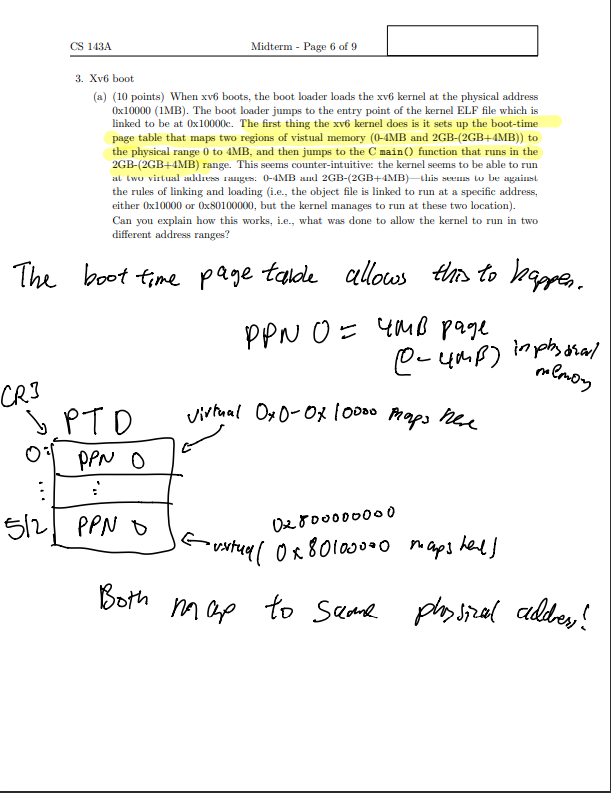
\includegraphics[width=0.5\columnwidth]{figs/point-3a}
\vfill

\end{parts}

\newpage

\addpoints 

\question Relocation

Alice compiles the following C file. 

\begin{verbatim}
#include<stdio.h>

int add (int a, int b) {
    printf("Numbers are added together\n");
    return a+b;
}

int main() {
    int a,b;
    a = 3;
    b = 4;

    int ret = add(a,b);

    printf("Result: %u\n", ret);
    return 0; 
}
\end{verbatim}


\begin{parts}

\part[5] Which symbols are undefined and need to be resolved (explain your answer)? 

\textbf{STUDENT SOLUTION } 
(NOT SURE) 


\begin{adjustwidth}{1.5em}{1em}
add() is undefined b/c not static\newline
printf() undefined as library func\newline
main() is undefined as non static function\newline
  
\end{adjustwidth}
\vfill
	
\newpage

\part[5] Which symbols need to be relocated? Note, that C treats string constants as globals allocated in the read-only 
	data section. Explain your answer. 

\textbf{STUDENT SOLUTION } 
(NOT SURE) 
\begin{adjustwidth}{1.5em}{1em}
add() is undefined b/c not static\newline
printf() undefined as library func\newline
main() is undefined as non static function\newline

"Num.." is undefined as run time allocated value\newline
"Res.." is undefined as run time allocated value\newline
  
\end{adjustwidth}
\vfill


\end{parts}

\end{questions}
\end{document}
